% !TEX program = xelatex
\documentclass[a4paper,12pt]{ctexart}

% 页面设置 — 遵循旧 Word 格式
\usepackage[a4paper,top=2.0cm,bottom=2.0cm,left=1.8cm,right=1.8cm]{geometry}

% 必要宏包
\usepackage{graphicx}
\usepackage{booktabs}
\usepackage{amsmath}
\usepackage{amssymb}
\usepackage{hyperref}
\usepackage{xcolor}
\usepackage{multirow}
\usepackage{array}
\usepackage{tabularx}
\usepackage{float}
\usepackage[numbers,sort&compress]{natbib}

% 图表路径
\graphicspath{{figures/}}

% 超链接设置
\hypersetup{
    colorlinks=true,
    linkcolor=black,
    citecolor=black,
    urlcolor=blue
}

% 标题
\title{时空深度学习模型在玉米—大豆分类中的空间泛化能力分析}
\author{}
\date{}

\begin{document}

\maketitle

% !TEX root = ../main.tex

\section{引言}

% 待迁移：旧稿引言（P020–P025）
% 当前为结构占位，正文内容待从旧稿迁移

% !TEX root = ../main.tex

\section{研究区域与数据}

\subsection{研究区概况}

本文选取美国中西部玉米带内4个典型农业站点作为研究区，分别记为A、B、C和D。4个站点中，A、B位于爱荷华州，C位于印第安纳州，D位于伊利诺伊州，单个站点空间范围约为77~km~$\times$~77~km。该区域是美国重要的商品粮生产区，农田分布集中，种植类型以玉米和大豆为主，适合开展玉米大豆时空深度学习模型遥感识别及空间泛化能力分析。研究区空间位置如图1所示。

为分析研究区地表覆盖组成，本文采用美国农业部国家农业统计服务局发布的耕地数据层（Cropland Data Layer，CDL）数据。基于2021—2024年CDL数据统计结果，4个站点均以玉米和大豆为主要作物类型，两者面积之和均超过农作物总面积的95\%。本文将CDL原始类别重分类为玉米、大豆和其它3类，其中除玉米和大豆以外的农作物和非农作物地类都归并为"其它地物"，标记为其它。

\begin{figure}[tbp]
\centering
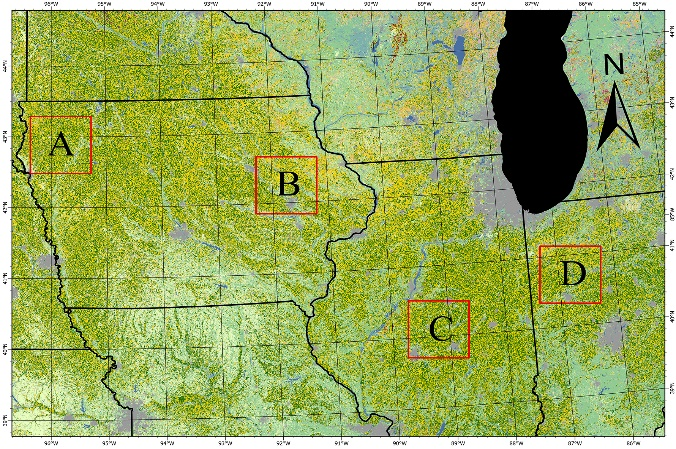
\includegraphics[width=\linewidth]{study_area/study_area.jpg}
\caption{研究区域4个站点分布图}
\label{fig:study_area}
\end{figure}

玉米和大豆物候信息来自美国农业部国家农业统计服务发布的作物进度报告（Crop Progress Report, CPR），其数据通过USDA NASS官网获取。结合CPR物候信息，本文将每年DOY~116—266作为主要观测窗口，该时间范围能够覆盖玉米和大豆的主要生育阶段。

\subsection{数据获取与预处理}

本文采用的多时相遥感数据源自美国国家航空航天局（NASA）地球数据科学系统提供的协同陆地卫星和哨兵2号数据（Harmonized Landsat and Sentinel-2，HLS）第2版。该产品通过对Landsat-8/9 OLI与Sentinel-2 MSI的观测影像进行辐射定标、大气校正、几何精校正以及网格重采样，实现了两类卫星数据的深度融合。本研究选取其空间分辨率为30~m的多时相地表反射率数据，包含蓝光、绿光、红光、近红外、短波红外1和短波红外2共6个核心波段作为深度学习模型的输入特征。

标签数据采用USDA NASS CropScape门户网站提供的2023年CDL产品。CDL数据提供了美国本土逐像素的年度作物类型分类信息，在本研究中用于模型训练的真值标记与精度检验。研究对原始的CDL分类体系进行重分类，统一划分为玉米（Corn）、大豆（Soybean）和其它（Others）3个目标类别。重分类后的标签数据在空间投影和分辨率上与对应的多时相HLS影像进行严格对齐。

在预处理阶段，首先对影像进行镶嵌、云掩膜和裁剪处理。随后，对时间序列采用时序线性插值方法补齐无效观测，并统一4个站点的时间跨度与时间间隔。最终，构建得到空间大小为2560$\times$2560像素，时间分辨率为5天、包含31个时间步、空间分辨率为30~m、光谱波段数为6的数据集。样本构建时，将多时相影像及其对应标签裁剪为128~$\times$~128像素图块，相邻图块无重叠；在此基础上，最终每个站点每年获得400个样本用于后续模型训练与验证。

\subsection{研究区空间特征}

本文基于2023年CDL参考标签，从地物组成和景观格局两个方面比较4个站点的空间特征，为后续站内分类与跨站比较提供研究区背景。

\subsubsection{地物组成}

如图\ref{fig:sec13_composition}所示，4个站点均以玉米和大豆为主要地物，两者面积之和占各站总面积的65.57\%～82.16\%。各站玉米面积占比为39.97\%～45.39\%，大豆占比为23.49\%～36.77\%，站点间大豆占比的变化幅度更大。A站两种作物合计占比最高，其它地物仅占17.84\%；B站大豆占比最低，其它地物占比达到34.43\%。因此，4个站点具有相同的主要作物组成，但两种作物与其它地物的面积配置存在差别。

\begin{figure}[tbp]
\centering
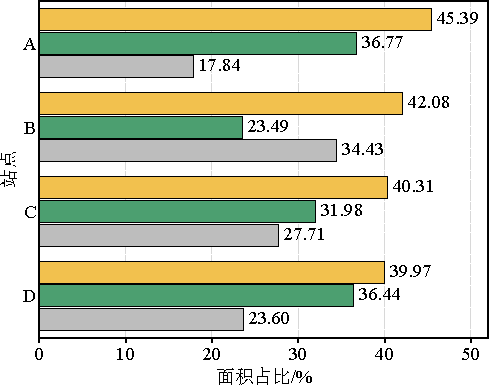
\includegraphics{study_area/fig_sec13_composition.pdf}
\par\nointerlineskip\vspace{3pt}
\classlegend
\caption{四个研究站点2023年地物面积占比}
\label{fig:sec13_composition}
\end{figure}

\subsubsection{景观格局}

本文采用FRAGSTATS计算完整参考斑块的面积（AREA）和形状指数（SHAPE）\citep{mcgarigal2023fragstats}。在各站2023年参考标签上，以8邻域相连的同类像元构成一个参考斑块。AREA表示斑块面积，SHAPE反映斑块边界相对于同面积紧凑形状的复杂程度。为避免大量微小斑块掩盖主要作物面积所在的斑块特征，分别按斑块等权和参考像元面积加权统计两项指标的分布；前者描述单个斑块的常见情况，后者描述随机取一个作物参考像元时其所在斑块的特征。

如表\ref{tab:sec13_patch_distribution}所示，按斑块等权统计，8组作物斑块的AREA中位数均仅为0.09～0.18~ha，SHAPE中位数均为1.00，反映出完整标签中存在大量细小且规则的斑块。按参考像元面积加权后，AREA中位数升至63.27～130.95~ha，说明主要作物面积集中在较大斑块中。C站玉米和大豆的面积加权SHAPE中位数分别为2.07和1.91，高于其余站点；A站分别为1.63和1.58。B站大豆的面积加权AREA中位数为63.27~ha，是8组中最低。两种权重下的数值差异表明，比较研究区斑块格局时需要同时考虑斑块数量和其承载的作物面积。

\begin{table*}[tbp]
\centering
\caption{四个研究站点2023年玉米和大豆完整参考斑块的AREA与SHAPE分布}
\label{tab:sec13_patch_distribution}
\begingroup
\songti\zihao{-5}
\setlength{\tabcolsep}{2pt}
\renewcommand{\arraystretch}{1.08}
\begin{tabular*}{\textwidth}{@{\extracolsep{\fill}}ccccccc@{}}
\toprule
\multirow{2}{*}{站点} & \multirow{2}{*}{地物类型} & \multirow{2}{*}{斑块数} & \multicolumn{2}{c}{AREA/ha} & \multicolumn{2}{c}{SHAPE} \\
\cmidrule(lr){4-5}\cmidrule(l){6-7}
 & & & 斑块等权 & 面积加权 & 斑块等权 & 面积加权 \\
\midrule
\csname @@input\endcsname tables/sec13_patch_distribution_rows.tex
\bottomrule
\end{tabular*}
\par\nointerlineskip\vspace{3pt}
\raggedright 注：数值为中位数（Q25～Q75）；面积加权以斑块包含的参考像元数为权重；SHAPE无量纲。
\par
\endgroup
\end{table*}

% !TEX root = ../main.tex

\section{研究方法}

\subsection{时空深度学习模型}

\subsubsection{U-TAE模型}

% 待重写

\subsubsection{3D U-Net模型}

% 待重写

\subsubsection{ConvGRU模型}

% 待重写

\subsection{实验设计}

本研究围绕玉米、大豆与其它三类目标，设计站内分类实验与跨站点空间泛化实验，以评估三种时空深度学习模型的分类能力与空间泛化性能。

\subsubsection{站内分类实验}

在站内实验中，每个站点使用2023年多时相HLS影像和CDL标签构建的400个非重叠图块样本，采用5折交叉验证策略进行模型训练与评估。具体而言，400个样本被划分为5个互不重叠的子集，每轮实验选取其中3个子集用于训练、1个子集用于验证（早停判断）、1个子集用于测试。重复5轮后，每个样本恰好被测试一次，形成完整的站内Out-of-Fold（OOF）预测。

站内结果从两个层面进行汇报。其一，将5轮测试各自计算的分类指标取均值与标准差，反映模型在不同训练-测试划分下的性能波动；其二，将5轮测试的混淆矩阵逐元素汇总后重新计算各项指标，得到基于完整OOF预测的总体精度，用于后续与跨站点结果进行一致口径的比较。

三种模型均基于PyTorch框架实现，采用统一的训练策略与超参数设置：优化器为AdamW，损失函数为交叉熵损失，初始学习率设为0.0001，批次大小为4，使用余弦退火学习率调度策略（$T_{\max}=50$，$\eta_{\min}=0.00005$），权重衰减为0.00005，梯度裁剪阈值为5.0，并引入早停机制（容忍轮次为15，最小改善量为0.0001）以防止过拟合。训练阶段对每个原始图块施加$0^{\circ}$、$90^{\circ}$、$180^{\circ}$和$270^{\circ}$四种旋转增强，使每折的有效训练样本量从240扩展至960。所有模型均在相同硬件环境下进行训练。

\subsubsection{跨站点空间泛化实验}

在跨站点泛化实验中，依次选取四个站点之一作为源站点，利用其站内实验训练所得的5个fold模型，分别对其余三个目标站点的全部400个图块进行逐图块推理。每条迁移路径产生5次独立的完整预测，对每次预测将400个图块的混淆矩阵汇总后计算各项指标，再对5次结果取均值与标准差。迁移过程中不对模型进行微调或集成，以评估模型结构本身的空间泛化能力。4个站点轮换作为源站点，共构成12条有向迁移路径，对应3种模型共36组结果、180次推理。

为量化跨站点应用的精度损失，本文以同一模型在目标站点的站内OOF汇总精度为参照基准，定义泛化退化指标（以玉米F1为例）：
\begin{equation}
\Delta\text{F1}_{\text{corn}} = \text{F1}_{\text{corn,within}} - \text{F1}_{\text{corn,cross}}
\end{equation}
其中$\text{F1}_{\text{corn,within}}$为该模型在目标站点的站内OOF汇总玉米F1分数，$\text{F1}_{\text{corn,cross}}$为源站点模型在目标站点的跨站点玉米F1五折均值，正值表示精度下降。大豆泛化退化$\Delta\text{F1}_{\text{soybean}}$同理计算。

\subsection{精度评价指标}

模型性能评估基于预测结果与像素级真实标签构建的混淆矩阵。对于三分类问题（玉米、大豆、其他），混淆矩阵元素$C_{ij}$表示真实类别为$i$但被预测为类别$j$的像元数。基于混淆矩阵，各类别F1分数计算如下：
\begin{equation}
\text{Precision}_i = \frac{C_{ii}}{\sum_{j} C_{ji}}, \quad
\text{Recall}_i = \frac{C_{ii}}{\sum_{j} C_{ij}}, \quad
\text{F1}_i = \frac{2 \cdot \text{Precision}_i \cdot \text{Recall}_i}{\text{Precision}_i + \text{Recall}_i}
\end{equation}
其中$i$为类别索引。总体精度（OA）定义为：
\begin{equation}
\text{OA} = \frac{\sum_{i} C_{ii}}{\sum_{i,j} C_{ij}}
\end{equation}

由于本研究的核心关注点是玉米和大豆的识别与泛化能力，本文分别报告玉米F1（$\text{F1}_{\text{corn}}$）和大豆F1（$\text{F1}_{\text{soybean}}$）作为主要评价指标。同时计算OA作为总体性能参考。

为检验不同模型的跨区域泛化性能是否存在统计学上的显著差异，本文将12条迁移路径作为配对单位，分别对三种模型的玉米F1和大豆F1进行Friedman非参数检验，并在总体差异显著时采用Wilcoxon符号秩检验进行两两比较，使用Holm方法校正多重检验。

\subsection{硬件和软件配置}

建模过程是在Linux工作站（Ubuntu 22.04）上进行的，该工作站具有一个Intel Xeon Gold 6430处理器（2.1~GHz/32 Core/60~M），120~GB RAM和1个NVIDIA GeForce RTX 4090显卡（24~GB RAM）。所有模型都使用PyTorch库实现。

% !TEX root = ../main.tex

\section{实验结果与分析}

\subsection{模型站内分类性能}

% 数据：results/summary/within_site_crop_f1.csv（汇总口径）、within_site_crop_f1_fold_stats.csv（折间 std）
% 数字核对 2026-09-19：范围、最大差值、折间 std 均与 csv 一致

如图\ref{fig:within_site_f1}所示，三种模型在四个站点的站内玉米F1为90.98\%～96.23\%，大豆F1为89.55\%～95.89\%。三种模型表现出两点共性：一是在同一站点，玉米F1均高于大豆F1，差值为0.09～1.88个百分点；二是在不同站点之间，玉米和大豆F1均在A站点达到各自最高值。五折交叉验证中，12组实验（3种模型×4个站点）的玉米F1折间标准差为0.12～0.73个百分点，大豆F1为0.06～0.96个百分点，表明各模型的站内作物分类表现稳定。

\par\addvspace{3pt}
\noindent\begin{minipage}{\linewidth}
\captionsetup{type=figure}
\centering
\begin{subfigure}{\linewidth}
\centering
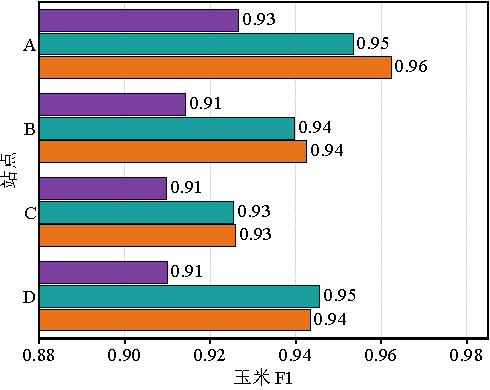
\includegraphics{results/fig_within_site_f1_a.pdf}
\caption{四站点玉米分类精度}
\end{subfigure}\par\nointerlineskip\vspace{3pt}
\begin{subfigure}{\linewidth}
\centering
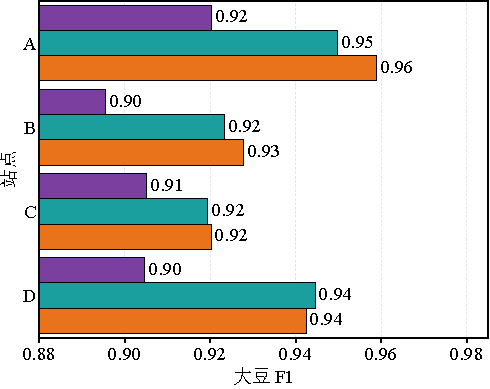
\includegraphics{results/fig_within_site_f1_b.pdf}
\caption{四站点大豆分类精度}
\end{subfigure}\par\nointerlineskip\vspace{3pt}
\modellegend
\caption{三种模型在四个站点的站内玉米和大豆分类精度}
\label{fig:within_site_f1}
\end{minipage}\par\addvspace{3pt}

三种模型之间存在较为稳定的精度差异。U-TAE和3D U-Net在各站点的玉米和大豆F1均高于ConvGRU，而U-TAE与3D U-Net之间的差值不超过1个百分点，二者互有高低：U-TAE在A、B、C三个站点略优，3D U-Net在D站点略优。ConvGRU的劣势幅度因站点而异：在C站点，三种模型的玉米和大豆F1最大差值分别为1.61和1.50个百分点；在D站点，该差值分别扩大至3.58和3.98个百分点。图\ref{fig:within_site_map_D}以D站点为例，直观对比了三种模型的站内交叉验证分类结果。以选中局部区域为例，ConvGRU的玉米和大豆像元错误率为12.1\%，明显高于3D U-Net（5.8\%）和U-TAE（4.8\%）。

% 图 3：上行全站 2560×2560 标红框，下行红框窗口放大；窗口 = D 站图块网格 (13,8) 起 2×2，像元行 1664–1920、列 1024–1280
% 选窗标准：只看真实玉米/大豆像元——作物像元错误率 ConvGRU 12.1% / 3D U-Net 5.8% / U-TAE 4.8%；
%   类别边界带错误率 32.0% / 15.3% / 13.4%；玉米↔大豆互混 6.8% / 2.6% / 2.2%。全站总错误率 10.6% / 6.3% / 6.7%
% 三模型 reference.tif sha256 一致（38ad33ef…）；oof_prediction.tif 为五折拼接，每图块预测来自未训练过它的模型

\begin{figure*}[tbp]
\centering
\begin{subfigure}{0.24\textwidth}\centering
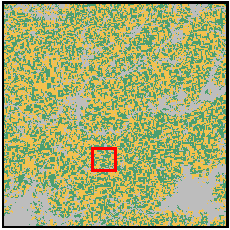
\includegraphics{results/fig_within_site_map_D_a.pdf}
\caption{参考标签}
\end{subfigure}\hfill
\begin{subfigure}{0.24\textwidth}\centering
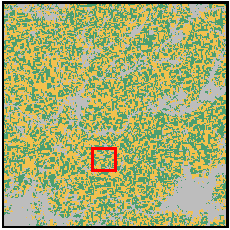
\includegraphics{results/fig_within_site_map_D_b.pdf}
\caption{ConvGRU分类结果}
\end{subfigure}\hfill
\begin{subfigure}{0.24\textwidth}\centering
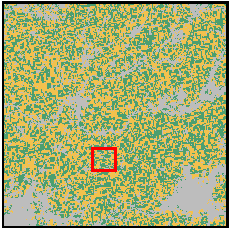
\includegraphics{results/fig_within_site_map_D_c.pdf}
\caption{3D U-Net分类结果}
\end{subfigure}\hfill
\begin{subfigure}{0.24\textwidth}\centering
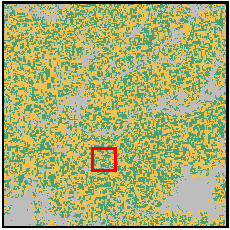
\includegraphics{results/fig_within_site_map_D_d.pdf}
\caption{U-TAE分类结果}
\end{subfigure}\par\nointerlineskip\vspace{3pt}
\begin{subfigure}{0.24\textwidth}\centering
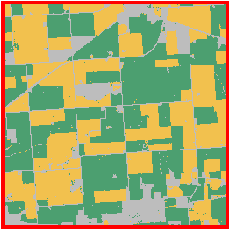
\includegraphics{results/fig_within_site_map_D_e.pdf}
\caption{参考标签}
\end{subfigure}\hfill
\begin{subfigure}{0.24\textwidth}\centering
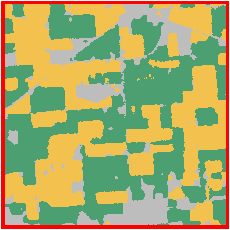
\includegraphics{results/fig_within_site_map_D_f.pdf}
\caption{ConvGRU分类结果}
\end{subfigure}\hfill
\begin{subfigure}{0.24\textwidth}\centering
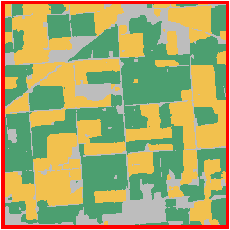
\includegraphics{results/fig_within_site_map_D_g.pdf}
\caption{3D U-Net分类结果}
\end{subfigure}\hfill
\begin{subfigure}{0.24\textwidth}\centering
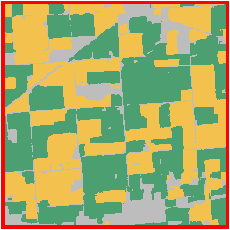
\includegraphics{results/fig_within_site_map_D_h.pdf}
\caption{U-TAE分类结果}
\end{subfigure}\par\nointerlineskip\vspace{3pt}
\classlegend
\caption{D站点三种模型站内交叉验证分类结果（上：全站，红框为局部窗口；下：局部窗口放大）}
\label{fig:within_site_map_D}
\end{figure*}

\FloatBarrier

\subsection{模型跨站分类性能与泛化退化}

% 数据：tables/table2_cross_site_f1_12paths.csv ← results/summary/cross_site_crop_f1_summary.csv（36 个模型—路径组合，5 次预测均值）
%       results/summary/within_site_crop_f1.csv（目标站站内汇总 F1，退化比例分母）
%       results/summary/crop_f1_relative_degradation_36paths.csv（图 4，泛化退化比例）
% 数字 2026-09-27 从上述文件现算；第一段范围取表内 36 格，最高值、最低值所在路径按模型逐一核对。

表\ref{tab:cross_site_f1_paths}给出了三种模型在12条迁移路径上的跨站玉米和大豆F1，每项为五次完整目标站预测的均值。源站模型不经微调直接用于目标站后，玉米F1为85.68\%～92.92\%，大豆F1为83.08\%～92.15\%，36个模型—路径组合的玉米和大豆F1均低于同一模型在目标站的站内汇总F1。按模型分别比较各条路径，三种模型的玉米和大豆跨站F1最高值均出现在以A站点为目标站的路径上，与站内结果中A站点精度最高相对应；三种模型的玉米跨站F1最低值则均出现在以C站点为目标站的路径上。

\begin{table*}[tbp]
\centering
\caption{三种模型在12条迁移路径上的跨站玉米和大豆F1}
\label{tab:cross_site_f1_paths}
{\songti\zihao{-5}
\renewcommand{\arraystretch}{1.12}
\setlength{\tabcolsep}{7pt}
\begin{tabular*}{\textwidth}{@{\extracolsep{\fill}}c*{6}{c}}
\toprule
\multirow{2}{*}{迁移路径} & \multicolumn{2}{c}{ConvGRU} & \multicolumn{2}{c}{3D U-Net} & \multicolumn{2}{c}{U-TAE} \\
\cmidrule(lr){2-3}\cmidrule(lr){4-5}\cmidrule(lr){6-7}
 & 玉米F1/\% & 大豆F1/\% & 玉米F1/\% & 大豆F1/\% & 玉米F1/\% & 大豆F1/\% \\
\midrule
A→B & 89.91 ± 0.11 & 87.52 ± 0.40 & 91.43 ± 0.39 & 89.28 ± 0.40 & 92.09 ± 0.26 & 89.90 ± 0.38 \\
A→C & 86.97 ± 0.59 & 86.94 ± 1.20 & 87.71 ± 0.59 & 87.96 ± 0.34 & 88.20 ± 0.61 & 88.29 ± 0.69 \\
A→D & 88.54 ± 0.67 & 88.05 ± 1.16 & 90.64 ± 0.53 & 90.56 ± 0.45 & 91.78 ± 0.43 & 91.48 ± 0.41 \\
B→A & 92.00 ± 0.18 & 91.59 ± 0.13 & 92.92 ± 0.59 & 92.15 ± 0.44 & 92.70 ± 0.25 & 91.87 ± 0.31 \\
B→C & 85.68 ± 0.95 & 84.52 ± 1.63 & 88.09 ± 0.55 & 88.20 ± 0.81 & 87.70 ± 0.58 & 87.66 ± 0.84 \\
B→D & 85.73 ± 1.67 & 83.08 ± 2.70 & 90.87 ± 0.33 & 90.43 ± 0.41 & 89.59 ± 1.41 & 88.50 ± 2.20 \\
C→A & 90.31 ± 0.59 & 90.15 ± 0.49 & 92.09 ± 0.40 & 91.64 ± 0.43 & 91.52 ± 0.61 & 91.09 ± 0.39 \\
C→B & 87.47 ± 1.05 & 85.06 ± 0.96 & 90.23 ± 1.00 & 88.98 ± 0.88 & 90.33 ± 0.62 & 88.18 ± 0.52 \\
C→D & 89.77 ± 0.29 & 89.57 ± 0.08 & 90.77 ± 0.85 & 90.91 ± 0.17 & 90.98 ± 0.39 & 90.70 ± 0.48 \\
D→A & 91.05 ± 0.24 & 90.85 ± 0.52 & 91.36 ± 0.68 & 91.32 ± 0.68 & 91.45 ± 0.26 & 92.04 ± 0.37 \\
D→B & 89.44 ± 0.24 & 86.19 ± 0.46 & 88.13 ± 1.24 & 86.19 ± 1.91 & 90.45 ± 0.45 & 89.17 ± 0.98 \\
D→C & 87.85 ± 0.30 & 88.19 ± 0.54 & 87.88 ± 0.71 & 88.60 ± 0.83 & 87.83 ± 0.89 & 88.41 ± 0.84 \\
\midrule
平均 & 88.73 & 87.64 & 90.18 & 89.69 & 90.39 & 89.77 \\
\bottomrule

\end{tabular*}
\par\nointerlineskip\vspace{3pt}
\begin{minipage}{\textwidth}
\noindent 注：箭头左侧为源站，右侧为目标站。每格为源站5个折模型分别预测目标站全部400个图块所得F1的算术平均，未进行微调和模型集成；“平均”为12条迁移路径F1均值的算术平均。
\end{minipage}
}
\end{table*}

% 第二段：12 条路径平均跨站 F1（表末行）；平均泛化退化比例 = 12 条路径比例的算术平均。
% 两种排序分别对应实际精度与相对同一模型目标站当地训练基准的差距。

按12条路径取算术平均，ConvGRU的跨站玉米和大豆F1分别为88.73\%和87.64\%，均低于3D U-Net（90.18\%、89.69\%）和U-TAE（90.39\%、89.77\%）。但同样对12条路径的泛化退化比例取算术平均，ConvGRU的玉米和大豆退化比例分别为3.05\%和3.32\%，小于3D U-Net（4.18\%、4.01\%）和U-TAE（4.21\%、4.22\%）。跨站F1反映模型在目标站的实际分类精度，泛化退化比例则衡量其与同一模型在目标站的站内汇总F1之间的相对差距。因此，泛化退化比例较小不代表跨站绝对精度更高，评价模型的跨站表现需要同时考察这两个指标。

% 第三段：图 4 数据 results/summary/crop_f1_relative_degradation_36paths.csv。
% 固定目标站 D：ConvGRU 大豆 C→D 0.99%、B→D 8.17%。
% B↔D：ConvGRU 玉米、大豆均 B→D 较大，3D U-Net 均 D→B 较大；比较基于各路径五次预测均值。

如图\ref{fig:degradation_heatmap}所示，按每条路径五次预测的F1均值计算的泛化退化比例随源—目标组合变化，不同模型的变化也不一致。固定D站点为目标站，ConvGRU的大豆泛化退化比例在源站为C时为0.99\%，源站为B时为8.17\%。在B、D两个站点之间，ConvGRU的玉米和大豆泛化退化比例均为B→D方向较大，3D U-Net则均为D→B方向较大；以大豆为例，ConvGRU在B→D和D→B路径上分别为8.17\%和3.75\%，3D U-Net分别为4.26\%和6.65\%。这一方向差异描述的是该站点对的均值表现，不代表普遍的迁移规律。这些路径差异的空间解释，还需结合各站点的地物组成与景观结构。

\begin{figure*}[tbp]
\centering
\begin{subfigure}{\dimexpr(\textwidth-6pt)/3\relax}\centering
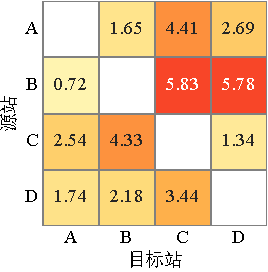
\includegraphics{results/fig_degradation_heatmap_a.pdf}
\caption{ConvGRU玉米泛化退化比例}
\end{subfigure}\hspace{3pt}%
\begin{subfigure}{\dimexpr(\textwidth-6pt)/3\relax}\centering
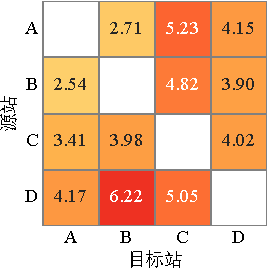
\includegraphics{results/fig_degradation_heatmap_b.pdf}
\caption{3D U-Net玉米泛化退化比例}
\end{subfigure}\hspace{3pt}%
\begin{subfigure}{\dimexpr(\textwidth-6pt)/3\relax}\centering
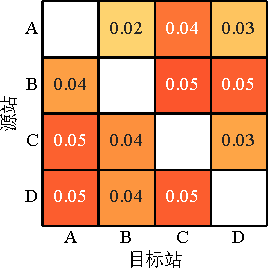
\includegraphics{results/fig_degradation_heatmap_c.pdf}
\caption{U-TAE玉米泛化退化比例}
\end{subfigure}\par\nointerlineskip\vspace{3pt}
\begin{subfigure}{\dimexpr(\textwidth-6pt)/3\relax}\centering
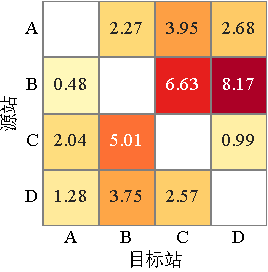
\includegraphics{results/fig_degradation_heatmap_d.pdf}
\caption{ConvGRU大豆泛化退化比例}
\end{subfigure}\hspace{3pt}%
\begin{subfigure}{\dimexpr(\textwidth-6pt)/3\relax}\centering
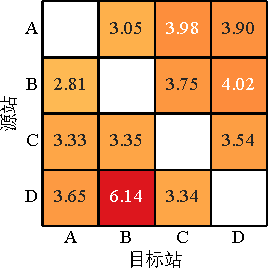
\includegraphics{results/fig_degradation_heatmap_e.pdf}
\caption{3D U-Net大豆泛化退化比例}
\end{subfigure}\hspace{3pt}%
\begin{subfigure}{\dimexpr(\textwidth-6pt)/3\relax}\centering
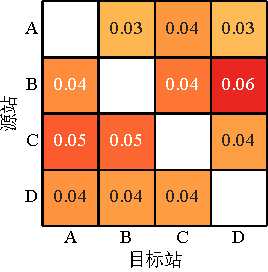
\includegraphics{results/fig_degradation_heatmap_f.pdf}
\caption{U-TAE大豆泛化退化比例}
\end{subfigure}\par\nointerlineskip\vspace{3pt}
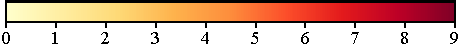
\includegraphics{results/fig_degradation_heatmap_cbar.pdf}\par\nointerlineskip\vspace{3pt}
{\songti\zihao{-5}泛化退化比例/\%\par}
\caption{不同源—目标区域组合下三种模型的玉米和大豆F1泛化退化比例（行为源站，列为目标站，对角线不适用）}
\label{fig:degradation_heatmap}
\end{figure*}

\FloatBarrier
\subsection{模型跨站泛化差异的空间解释}

% 数据（已生成，未入库）：图块级 D:/cross_site_all_20260916/paper_tables/Patch级空间误差底表/ 四张表；
%   站点级 D:/label/fragstats_results/完整标签{景观级,类别级}指标.csv（2023 年标签，ED 为景观级，AREA_MN、AI 为类别级）
% 方法：按空间特征分组后汇总混淆矩阵再算类别 F1；跨站逐次计算后再汇总 5 次结果，站内以同组图块为参照；不平均图块 F1
% 两个问题，覆盖全部站点与 12 条路径：目标站哪些空间条件下退化较大；同一目标站的退化随源站的变化与站点间哪些差异相对应

% !TEX root = ../main.tex

\section{讨论}

% 旧稿中讨论部分较薄，主要融合在结论和结果分析中
% 待根据 plan/outline.md 新建讨论结构

% !TEX root = ../main.tex

\section{结论}


\bibliographystyle{unsrtnat}
\bibliography{bibliography/references}

\end{document}
